\documentclass[12pt, oneside]{article}
\usepackage[letterpaper, margin=1in, headsep=0.5in, left=0.3in, right=2.5in]{geometry}
\usepackage[english]{babel}
\usepackage[utf8]{inputenc}
\usepackage{amsmath}
\usepackage{amsfonts}
\usepackage{amssymb}
\usepackage{tikz}
\usepackage{yhmath}
\usetikzlibrary{quotes, angles}
\usepackage{graphicx}
\usepackage{enumitem}
\usepackage{multicol}

\newif\ifmeta
\metatrue %print standards and topics tags

\title{Regents Geometry}
\author{Chris Huson}
\date{May 2022}

\usepackage{fancyhdr}
\pagestyle{fancy}
\fancyhf{}
\renewcommand{\headrulewidth}{0pt} % disable the underline of the header
\raggedbottom

%\fancyhead[LE]{\thepage}
\fancyhead[RO]{Name:}
\fancyhead[LO]{BECA / Dr. Huson / Geometry Regents Mixed Review}
\cfoot{\thepage}

\begin{document}
\subsubsection*{11.12 External angles}
\begin{enumerate}[itemsep=1.2cm]
\item As shown below, triangle $ABC$ has $m\angle A = 52^\circ$ and $m\angle B = 48^\circ$. Find the measure of the external angle $\angle BCD = x$.
\begin{center}
  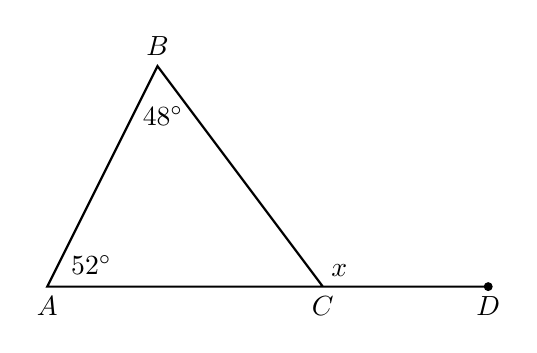
\begin{tikzpicture}[scale=0.7]
  \draw [thick]
  (10,0)node[below]{$D$}--
  (2,0)node[below]{$A$}--
  (4,4)node[above]{$B$}--
  (7,0)node[below]{$C$};
  \draw [fill] (10,0) circle [radius=0.07];
  %\draw [thick](2,0)node[below]{$E$}--(4,4);
  \node at (2.8,0.4){$52^\circ$};
  \node at (7.3,0.3){$x$};
  \node at (4.1,3.1){$48^\circ$};
\end{tikzpicture}
\end{center}

\item Given $\triangle ABC$ with $\overrightarrow{ACD}$.
\begin{center}
  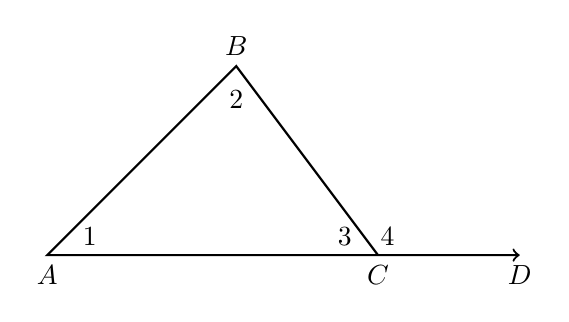
\begin{tikzpicture}[scale=0.6]
  \draw [thick, <-]
  (10,0)node[below]{$D$}--
  (0,0)node[below]{$A$}--
  (4,4)node[above]{$B$}--
  (7,0)node[below]{$C$};
  \node at (0.9,0.4){1};
  \node at (6.3,0.4){3};
  \node at (7.2,0.4){4};
  \node at (4,3.3){2};
\end{tikzpicture}
\end{center}
Which equation is always true?
\begin{multicols}{2}
\begin{enumerate}
  \item $m\angle 3 = m\angle 1 + m\angle 2$
  \item $m\angle 3 = m\angle 1 - m\angle 2$ 
  \item $m\angle 4 = m\angle 1 + m\angle 2$
  \item $m\angle 4 = m\angle 3 - m\angle 2$
\end{enumerate}
\end{multicols}

\item In  $\triangle ABC$ shown below, side $\overline{AC}$ is extended to point $D$ with $m\angle DAB=(180-2x)^\circ$, $m\angle C=(x-10)^\circ$, and $m\angle B=(3x+10)^\circ$.
\begin{center}
  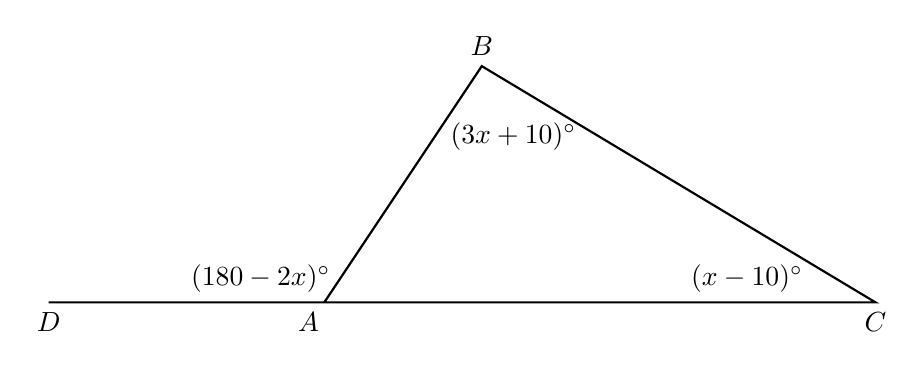
\begin{tikzpicture}
    \draw [thick](-1.5,0)node[below]{$D$}--
      (1.8,0)node[below]{$A$}--
      (9,0)node[below]{$C$}--
      (4,3)node[above]{$B$} --(2,0);
      \node at (2.2,0)[above left]{$(180-2x)^\circ$};
      \node at (8.2,0)[above left]{$(x-10)^\circ$};
      \node at (4.4,2.4)[below]{$(3x+10)^\circ$};
  \end{tikzpicture}
\end{center}
What is $m\angle BAC$?

\newpage
\item Randy's basketball is in the shape of a sphere with a maximum circumference of 29.5 inches. Determine and state the volume of the basketball, to the \emph{nearest cubic inch}.
\vspace{2cm}

\item What are the coordinates of the center and the length of the radius of the circle whose equation is $(x-6)^2+(y+8)^2=64$?
\vspace{1cm}

\item In a right triangle, the acute angles have the relationship \\$\sin (2x + 9)=\cos (x+12)$.\\[0.25cm]
What is the value of $x$?
\vspace{1cm}

\item As shown, circle $O$ has chords $\overline{AD}$ and $\overline{BE}$ intersecting at $C$, and $m \wideparen{AB}=72^\circ$, $m \wideparen{BD}=78^\circ$, $m \wideparen{AE}=94^\circ$, and $m \wideparen{DE}=116^\circ$. $BC=6.6$, $AC=8.8$, and $CE=13.2$.
  \begin{multicols}{2}
  \raggedcolumns
  \begin{flushright}
    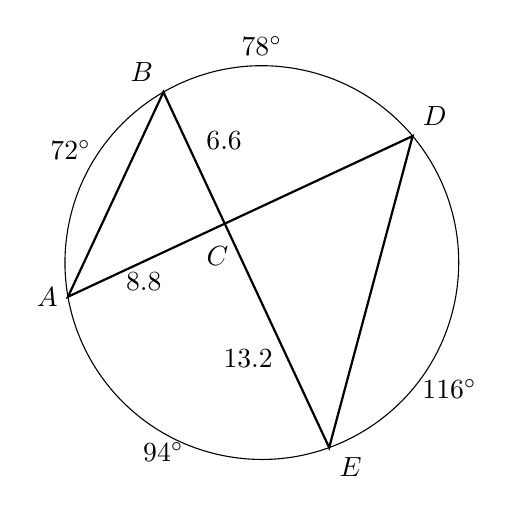
\begin{tikzpicture}[scale=.5, rotate=-10]
    \draw (0,0) circle[radius=5];
    \draw [thick]
    (-60:5) node[below right] {$E$}--
    (130:5) node[above left] {$B$}--
    (200:5) node[left] {$A$}--
    (50:5) node[above right] {$D$}--cycle;
    \draw (160:1.3) node[below] {$C$};
    \draw (115:3.7) node[below] {$6.6$};
    \draw (190:3) node[below] {$8.8$};
    \draw (270:2.0) node[below] {$13.2$};
    \draw (-30:5) node[right] {$116^\circ$};
    \draw (100:5) node[above] {$78^\circ$};
    \draw (155:5) node[left] {$72^\circ$};
    \draw (250:5) node[below] {$94^\circ$};
    \end{tikzpicture}
  \end{flushright}
  \begin{enumerate}
    \item Write down $m\angle B$, $m\angle D$. \vspace{0.5cm}
    \item Write down $m\angle A$, $m\angle E$. \vspace{0.5cm}
    \item Find $m\angle ACB$. \vspace{1.5cm}
    \item Find the scale factor and $CD$.
    \end{enumerate}
  \end{multicols}

\end{enumerate}
\end{document}
  